
\chapter{Related Work}
\label{chap:related_work}

This chapter introduces the basic concepts necessary to understand the models
and tools  used in this work. Section \ref{sec:deep_learning} introduces
basic concepts of deep learning and representation learning. After that, in
sections  \ref{sec:rel_nlp} to \ref{sec:sub_continuous_representation}
the basics of natural language processing and text representation  are
discussed. Sections \ref{sec:relwork-language-models} and \ref{sec:n-gram-lm} introduce statistical
language modeling and the classical $N$-gram based approach. Finally,
Section \ref{sec:nnlms-intro} explores 
  in detail some of the existing language  models based
on neural networks. The reason for this, is that continuous word vector
representation model used in this work, namely \textit{Word2vec}, relies
heavily on concept developed by these architectures. Thus, understanding  previous models  will help to understand the rationale and
motivation behind \textit{Word2vec}. 
\section{Deep Learning and Representation Learning}
 \label{sec:deep_learning}
Performance of machine learning methods relies heavily on the choices of the
data representation or features used to train the algorithm. Therefore,
choosing the right feature set is crucial when developing  machine learning
 systems. This step, generally part of a more complex processing
pipeline, is called feature engineering.
Although an important step, feature engineering is expensive in term of labor needed
to perform it successfully. Feature engineering generally requires   expert
knowledge of the application domain.  In order to expand the applicability
and speeding up the development of machine learning based systems, it would
be desirable to 
depend less on feature engineering by employing algorithms  that could extract
meaningful  information from raw input, turning this information into
features to be  used  in different machine learning settings.

Feature learning or representation learning is a set of techniques in machine
learning that learn a transformation from these raw inputs to a representation that
can be effectively exploited in a supervised learning task such as
classification \cite{DBLP:journals/corr/abs-1206-5538}. 
These representations  are learned by using several layers of
non-linearities, were each layer learns increasingly complex level of
representation.  However, high depth is
not a requirement to learn useful representation. Depending on the tasks
relatively shallow architectures produce useful features.

One important  concept in representation learning  is the concept of
\textit{distributed representations}.  A distributed representation is a representation  where $k$ 
out of $N$ representation elements or feature values cannot  be independently
varied, e.g., they are not mutually exclusive. K features being turned on or
active represent each concept while each feature is involved 
in representing many concepts \cite{DBLP:journals/corr/abs-1206-5538}.
There are many reasons for which having automatically learning distributed representations are
desirable to have.  First,  distributed representations enable to fight the \textit{ curse of
dimensionality} by capturing a huge number of possible input configurations in
reasonably sized learned representations. These representations often offer
similarity models that can be useful to improve existing algorithms.
Second,  handcrafting features is time consuming, and it often generates
over-specified and incomplete representation, requiring repeating  work when
switching tasks or  domains. Finally, many supervised  machine learning techniques
require labeled data while in domains the majority of data is unlabeled.  By learning
representations based on unlabeled data, this information can be harnessed
to learn powerful classifiers.



% In fact, the model used in
%this work to obtain word representations  can is not particulary deep,
%however two layers are used to obtain trh
%However, the ideas behind it were inspired from deep architectures.


% One way to obtain distributed representation of symbolic data is through the
% usage of neural network. Each layer of a neural network learns  through its
% weights representation useful for the following layer.



%PARAGRAPH INTRODUCING DISTRIBUTED REPRESENTATION

% A distributed representation is a concept that is central to connectionism.
% In a connectionist network, 
%A distributed representation occurs when some
%concept or meaning is represented by a  network, but that meaning is
% represented by a pattern of activity across a number of processing units
% (e.g. neurons in a neural network) 




%  In order to expand the scope
% and ease of applicability of machine learning, it would be
% highly desirable to make learning algorithms less dependent
% on feature engineering, so that novel applications could be
% constructed faster, and more importantly, to make progress
% towards Articial Intelligence (AI).


% *Avoid manual time consuming human work
% ***  Need for distributional and distributed representation
%       (Talk about what is everything)
%       Because distubuted represenation deal with the curse of dimensionality
%       (In orden to generalize properly in High dimensional space you need
%       representative examples for all relevant variations)
%       Alternatives to that are: 
%       - "Manual Feature Design".
%       - Assuming a smooth target
%       - Kernel methods (Linear in term of kernel based data points) - Get
%         into that.
%       - Unsupervised feature and weight learning.
     
% *** Using unlabeled data... most of the data we have access too is unlabeled. 
% *** Having multiple layers of representation (are more obvious for Computer layers)
% *** Why now?
%     Until 2006 were not able to torain to do something useful.
%     - New methods for doing unsiupervised learning. (RBM, AutoEnconders,
%       Constratctive Estimation)
%     - More efficient parameter stimation methods.
%     - Better understangin of model regularization.

\section{Natural Language Processing}
\label{sec:rel_nlp}
Natural language processing \ac{NLP} is a field of computer science,
artificial intelligence, and linguistics that studies efficient mechanisms to
provide natural language understanding and generation  machines. 
Statistical \ac{NLP} comprises all quantitative approaches to automated
language processing, including probabilistic modeling, information theory,
information theory and linear algebra \cite{Manning:1999:FSN:311445}.  Modern
\ac{NLP}  techniques make  use of  machine learning, data mining  and others data
driven techniques.

Major tasks of \ac{NLP} include  \ac{POS} (detecting part of speech in a
sentence), \ac{NER}  (Determining which items of a sentence map to proper
names, e.g. person, location, etc.),   Sentiment Analysis (Extracting
subjective information usually from a set of documents), among others. 
In some cases, sets of related tasks are grouped into subfields that are often
considered separately from \ac{NLP}. \ac{IR} is concerned with storing,
searching, and retrieving information, in particular  information stored as
text. Although considered a separate field, many tasks of \ac{IR} such a
\ac{TC} rely on \ac{NLP} methods. Thus, there is an overlap between the two
fields in several applications.



\section{Represenations of Text}
 \label{sec:rel_represenation_text}
  Many of the tasks of \ac{NLP} and \ac{IR} deal with textual data. Therefore
  the way  of representing this information is of key importance and affects
  directly the performance of the methods.  For  Statistical and machine
  learning techniques, these representations become the input features of
  such algorithms. Thus, using appropriate representation  becomes really
  important as the suitability of the representation  depends on the specific
  task.
  
  Text can be represented at several abstraction level.  The most of the
  common work at the document level, representing the complete document as a
  mathematical object (e.g. a vector). Other representation work based on
  sequence of words extracted from a text, i.e. $n$-grams or at word level
  (i.e. word vector embedding). Based on the characteristics of the
  representations they can be classified as local or continuous. 
 
  

\section{Local Representations}
 \label{sec:rel_local_representation}
A local representation is a vector of features that characterize the meaning
of the symbol. These features are mutually exclusive. That is, each feature
represents a unique characteristic.

\subsection{$N$-grams}
 \label{sec:sub_ngrams}

An $n$-gram is a sequence of $n$ items from given text corpus. The items can
be phonemes, syllables, letters or words. In this  work, the term
\textit{$n$-gram} refers only   to  word $n$-grams.
An $n$-gram of size 1 is referred to as a "unigram"; size 2 is a "bigram";
size 3 is a "trigram". Larger sizes are sometimes referred to by the value of
n. As the frequencies of the $n$-grams are of interest for statistical
modeling, the number of occurrences usually accompanies these
representations. This representation  have been used successful used in language modeling (see section
\ref{sec:relwork-language-models}). N-gram based language models have been  the dominant approach for
 language modeling since the 1980s \cite{Bengio:2008}.


% Note that in a simple n-gram language model, the probability of a word, conditioned on some number of previous words (one word in a bigram model, two words in a trigram model, etc.) can be described as following a categorical distribution (often imprecisely called a "multinomial distribution").

 \subsection{Bag-of-words (BOW)}
 \label{sec:rel_bow}

Bag of Word is a document level representation in which each document of a corpus is assigned a vector of dimensionality $V$, where $V$ is the
vocabulary of that corpus. Each component of this vector has an associated word of
the vocabulary. The values of each of the component can be binary, i.e. representing the
word occurrence or absence in the document, or a more sophisticated metric
such as \ac{tf-idf} \cite{Salton88term-weightingapproaches}.


Term frequency $tf_j$  is the number of times that a word $j$ appears in a
document $d$. The document frequency  $df_{j}$  is the number of documents
the term $j$ appears in the entire corpus.  With these two values,  \ac{tf-idf}  for a  word $j$ is  calculated as follows:

\begin{equation*}
  \label{eq:tf-idf}
  \text{tf-idf}_{j}=tf_{j}(d)\centerdot log(\frac{N}{df_{j}}),\,\,\,\,\forall
  j \in V
\end{equation*}

With $N$ the total number of documents in the document set.  This representation of text does not take  into account the actual order of the words inside the document. Despite
of that, it has  performed well in many \ac{IR} tasks (e.g. search, \ac{TC},
etc.) \cite{Sebastiani02}. Variations and extension of this technique are
still used in modern \ac{IR} systems.

 \subsection{1-of-N coding}
 \label{sec:1_of_coding}

 This is a word level representation. It is also called \textit{one hot
   representation}. The feature vector has the same length as the size of the
 vocabulary of the corpus. All the features or dimensions are zero but one.
 Representing a unique word of the vocabulary.            This representation is
 commonly used as an input for language models based on neural networks (see
 section \ref{sec:nnlms-intro}.)


 \section{Continuous Representations of Words}

\label{sec:sub_continuous_representation}
 Continuous representation  of words  can be divided between distributional and
 distributed representations. 

\subsection{Distributional Word Representations}

Distributional representations are based on the idea that a lot of
information can be obtained by representing a word by means of its neighbors.
Distributional representation are generally used to obtain document level representations.
Distributional word representations are based upon a cooccurrence matrix $F$
of size $V \times C$.  Each row of $F$ is the 
initial representation of a word $w$, and each column is some context
\cite{Turian:2010:WRS:1858681.1858721}. The context is  generally windows of
 words surrounding $w$. Each value of the context  represented using a type of
frequency count such as \ac{tf-idf}. Commonly used techniques for obtaining distributional
representations  are \ac{LSA} \cite{Dumais:1988:ULS:57167.57214} and \ac{LDA}
\cite{Blei:2003:LDA:944919.944937}.


 \subsubsection{Latent Semantic Analysis}
 \label{sec:rel_sa}
\ac{LSA} is the application of \ac{SVD} to a matrix where each row a document
represented using the \ac{BOW} model. In this way
 \ac{LSA} induce   distributional representations over F in which
each column is a document context \cite{Turian:2010:WRS:1858681.1858721}.  
One drawback of this technique is that,  for large databases the SVD
calculation becomes intractable, since the computation is extremely
expensive.

 \subsubsection{Latent Dirichlet Allocation}
 \label{sec:rel_lda}
\ac{LDA} is a generative probabilistic model of a corpus and the
idea behind it is that the documents are represented as weighted relevancy
vectors over latent topics, where a topic is characterized by a distribution over
words \cite{Blei:2003:LDA:944919.944937}.
Learning the various distributions (the set of topics, their associated word
probabilities, the topic of each word, and the particular topic mixture of
each document) is the objective of applying this topic modeling.

Similar to \ac{LSA} the result of \ac{LDA} is a lower dimensional
representation of the document. In particular, LDA
reduces the  to a fixed set of values  (i.e. a vector),  based on the
probability distribution of the words in the documents.

 \subsection{Distributed Representations}
 \label{sec:dis_rep}
The  advantages of  learning and using  distributed representation were already discussed in section \ref{sec:deep_learning}.
At the word level, distributed word representations assign a real-valued vector
to each word. As with other distributed representations, the  difference with
local representations lies  is that the representation mechanism, i.e. a single 
feature does not represent a single concept or relationship.
In the context of \ac{NLP}, Hinton  \cite{hinton:learndistrep} introduced distributed representations for textual data. 
 Bengio et al. \cite{Bengio:2008} combined distributed representations with neural network probability prediction  to apply them  to
statistical language model by through his
neural network based language model. Collobert  et al.\cite{collobert:2008}, Mhin et
al \cite{Mnih08ascalable} and
Mikolov et al.  \cite{conf/interspeech/MikolovKBCK10,conf/icassp/MikolovKBGC09} have further developed similar architectures focusing in improving the performance and estimation accuracy. Section \ref{sec:nnlms-intro} discusses some of these models with more detail.


% Distributed representation of words can be obtained from various neural
% network based language models and models inspired on them. 


% A distributed representation is a concept that is central to connectionism.
% In a connectionist network, a distributed representation occurs when some
% concept or meaning is represented by the network, but that meaning is
% represented by a pattern of activity across a number of processing units
% (e.g. neurons in a neural network) \cite{hinton:learndistrep}. 


% these are generally learned by neural network, where one of the layer of the
% network 

% Section blah blah will talk about directly and indirectly learn distributed
% representation of text using neural networks.



\section{Statistical Language Models}
\label{sec:relwork-language-models}

A statistical language model assigns a probability to a sequence of m
words $P(w_1,\ldots,w_m)$.  In most statistical language model it is assumed
that the probability of $i$-th word $w_t$ only depends on the sequence of the
$n-1$ previous word.  Using this assumption, the probability
$P(w_1,\ldots,w_m)$ can be calculated by \cite{Bengio:2008}: 
% 
%This probability can be obtained from the probability of
%each word given the context of words preceding it using the chain rule of probability 


\begin{equation}
\label{eq:lm_probability}
 P(w_1, w_2, \ldots, w_{t-1},w_t) = P(w_1) P(w_2|w_1) P(w_3|w_1,w_2) \ldots 
  P(w_t | w_1, w_2, \ldots w_{t-1}).
\end{equation}

Most probabilistic language models  approximate $P(w_t | w_1, w_2, \ldots
w_{t-1})$ using a fixed context of size $n-1$, i.e. using  $P(w_t |
w_{t-n+1}, \ldots w_{t-1})$.

Language model has applications in fields such speech recognition and data
compression, where the model tries to predict the next word in a speech
sequence. In the field of \ac{IR} language model are used generally 
to rank documents based on the probability that a language model would
generate terms from a specific query \cite{Manning:1999:FSN:311445}.

Although not in an extensively , this section covers existing statistical
language models. In particular, the dominant $n$-gram based model and other  models that
serve as basis for the architecture of  \textit{Word2vec} are discussed.
%  models that are related to \textit{Word2vec} are
%covered %
%Although this work only discusses statistical language model, there are
%other approaches to language modeling including  


\section{$N$-Grams based language models}
\label{sec:n-gram-lm}

The most frequently used language models are based on the n-gram statistics,
which are basically word co-occurrence
frequencies \cite{Manning:1999:FSN:311445} . The maximum likelihood estimate
of probability of word $A$ in context $H$ is then estimated by:


\begin{equation}
\label{eq:ngram-prob}
  P(A|H) = \frac{C(HA)}{C(H)}
\end{equation}

where $C(HA)$ is the number of times that the $HA$ sequence of words has
occurred in the training data. The context $H$ can consist of several words,
for the usual trigram models $|H| = 2$. For $H = 0$ , the model is called
unigram. The unigram model only models the word probability on the corpus,
and does not take into account historical information
\cite{Manning:1999:FSN:311445, mikolovphd2012}. 

As many of these probability estimates are going to be zero (for all words that were not seen in the training data in a particular context $H$), smoothing needs to be applied. This works by redistributing probabilities between seen and unseen (zero-frequency) events, by exploiting the fact that some estimates, mostly those based on single observations, are greatly over-estimated. 

% The other way around, building language models from huge amounts of data (hundreds
% of billion words or more) is also a very challenging task, and has received recently a lot
% of attention [26]. The problems that arise include smoothing, as well as compression
% techniques, because it is practically impossible to store the full n-gram models estimated
% from such amount of data in computer memory. While amount of text that is available
% on the Internet is ever-increasing and computers are getting faster and memory bigger, we
% cannot hope to build a database of all possible sentences that can ever be said.

\section{Maximum Entropy Language Models}
\label{sec:max-ent-lm}

\ac{ME} model is an exponential model with the following form :

\begin{equation}
  \label{eq:max-ent-prob}
   P(w|h) = \frac{e^{a_w}}{Z(h)}
\end{equation}

with $a_w$ defined as:

\begin{equation}
  \label{eq:max-ent-pro-sub1}
  a_w = \sum_{i}{\lambda_i f_i(w,h)} 
\end{equation}

where $w$ is a word in a context $h$ and $Z(h)$ is  the normalization factor:

\begin{equation}
  \label{eq:max-ent-prob-sub2}
  Z(h) = \sum_{w_i \in V}{e^{\sum{\lambda_{j} f_j(w,h)}}} 
\end{equation}

Where $f_i(w,h)$ are  the feature functions based on the word and its
context. Therefore, the problem of training a  \ac{ME} consiste of  find the
weights  $\lambda_i$ and select the features $f_i$, which are not learned from
the data. Usually, the features functions $f(w,h)$ for these  models are
$n$-grams probabilities. \ac{ME} models can
be seen as simple neural network without a hidden layer and can be trained
using stochastic gradient descent \cite{Bishop:1995:NNP:525960, mikolovphd2012}.


%\sum_{l=1}^N e^{a_l}


\section{Neural Network Language Models}
\label{sec:nnlms-intro}

As its name describes,  \ac{NNLM} are  language models based on Neural Networks, exploiting their
ability to learn distributed representations to reduce the impact of the
\textit{curse of dimensionality} \cite{Bengio:2008}. In other words, a \ac{NN} is
used to estimate the probability described  by equation (\ref{eq:lm_probability}) based on a sequence of
previous words.

The advantage  using  distributed representations  is that they allow
the model to generalize well to sequences that are not in the set of training
word sequences, but that are similar in terms of their features. Because neural networks tend to map nearby inputs
to nearby outputs, the predictions corresponding to word sequences with
similar features are mapped to similar predictions \cite{Bengio:2008,Bengio:2003:NPL:944919.944966}.

However, due to the nature the multilayer architecture common of neutral
network, \ac{NNLM}  suffer from  
performance issues, where the hidden layers and the output layer are
generally the bottleneck. In order to be able to compare the different
models in term of their computational complexity, it is necessary then to define it in
term of their architecture. For all the models discussed here, the  complexity proportional to \cite{DBLP:journals/corr/abs-1301-3781}:

\begin{center}
\begin{equation} O = E \times T \times Q,   \end{equation}
\end{center}

$E$ is number of the training epochs (i.e.  number of upasses through the entire training set) , $T$ is the number of the words in
the training set and $Q$ depends on each architecture. Common choice is $E$ = 3-50 and $T$ up to one billion.
All models are trained using stochastic gradient descent and backpropagation
\cite{Bengio:2003:NPL:944919.944966,DBLP:journals/corr/abs-1301-3781}.

The following section describes each of the most representative  models and their
associated complexity $Q$.


%%PUT RELATION TO WORK TO VEC HERE

\subsection{Feedforward Neural Network Language Model}
\label{subsec:fwd-neural-net-lm}

% Section \ref{sec:relwork-language-models} described the generalities of
% language models in the context of \ac{NLP}.  In that section we described
% that the  

In the \ac{FNNLM} introduced by Bengio
\cite{Bengio:2003:NPL:944919.944966},  the probabilistic prediction $P(w_t | w_{t-n+1}, \ldots w_{t-1})$ 
in equation (\ref{eq:lm_probability}) is obtained as follows. 
First, each word $w_t$ is associated to a one-hot verctor of dimension $V$ with an entry at postion $t$, and zeros otherwise.  Then each vector is mapped to a $d$-dim feature vector $C_{w_t}$. The feature vectors $C_w$ are interpreted as the columns of a parameter matrix $C$, which represents the linear transformation between the $V$-dimensional one-hot vectors and the $d$-dim feature vectors. 

%First, each word $w_{t-i}$ (represented
%with an integer in $[1,N]$) in the  $n-1$-word context is mapped
%$$to an associated $d$-dimensional feature vector $C_{w_{t-i}}\ ,$ which is
%$column $w_{t-i}$ of parameter matrix $C\ .$ 
Vector $C_{w_{k}}$ contains the learned features for word $k\ .$
Let the  vector $x$ denote the concatenation of these $n-1$
feature vectors:
\begin{equation}
  x = (C_{w_{t-n+1},1}, \ldots, C_{w_{t-n+1},d}, C_{w_{t-n+2},1}, \ldots C_{w_{t-2},d}, C_{w_{t-1},1}, \ldots C_{w_{t-1},d}).
\end{equation}
The probabilistic prediction of the next word, starting from $x$
is then obtained using a standard artificial neural network architecture
for probabilistic classification, using the softmax activation function at the output units \cite{Bishop:1995:NNP:525960}:
\begin{equation}
 P(w_t=k | w_{t-n+1}, \ldots w_{t-1}) = \frac{e^{a_k}}{\sum_{l=1}^N e^{a_l}}
\end{equation}
where
\begin{equation}
 a_k = b_k + \sum_{i=1}^h W_{ki} \tanh(c_i + \sum_{j=1}^{(n-1)d} V_{ij} x_j)
\end{equation}
where the vectors $b,c$ and matrices $W,V$ are also
parameters of the \ac{NN}  (in addition to matrix $C$). Let us denote
$\theta$ for the concatenation of all the parameters.
The number of hidden units $h$
and the number of learned word features $d$  control the  complexity of the model.


\begin{figure}[h]
    \centering
    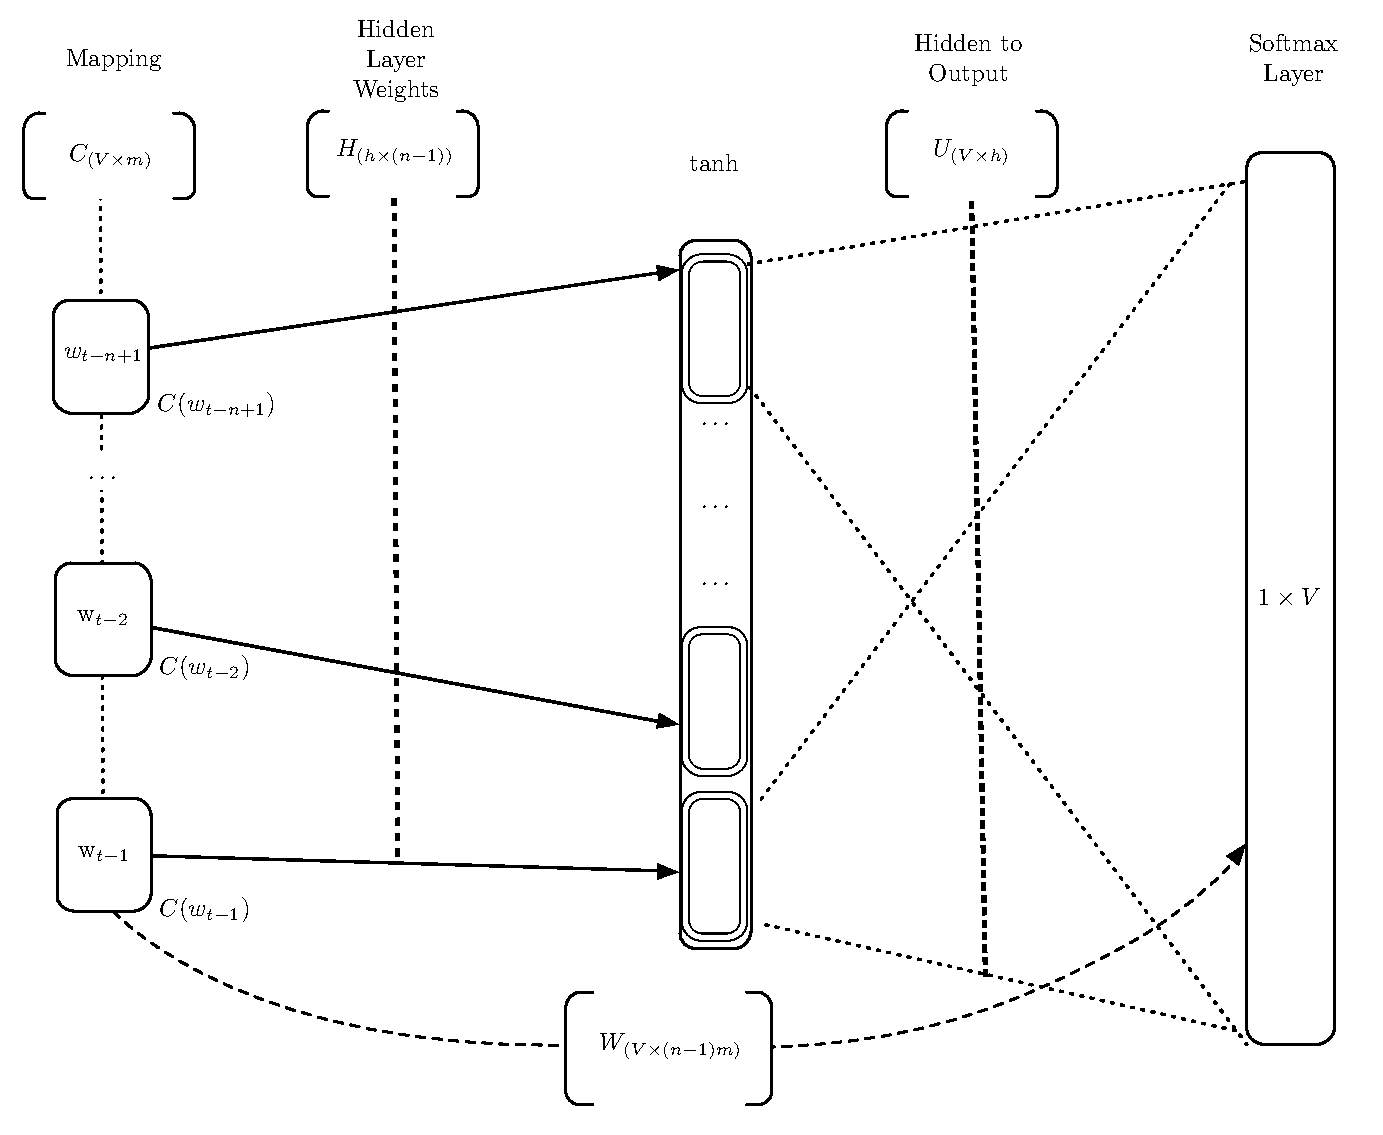
\includegraphics[width=0.7\textwidth]{images/bengio-nnlm.pdf}
    \caption{Feed Forward Neural Network Model Language Model Architecture.
       $C(i)$ is the $i$-th word feature vector.  \cite{Bengio:2003:NPL:944919.944966}.}
    \label{fig:NNLM_architecture}
\end{figure}

The neural network is trained using a gradient-based optimization algorithm
to maximize the training set \textit{log-likelihood}
\begin{equation}
 L(\theta) = \sum_t \log P(w_t | w_{t-n+1}, \ldots w_{t-1}) .
\end{equation}
The gradient $\frac{\partial L(\theta)}{\partial \theta}$
can be computed using the backpropagation algorithm \cite{Bishop:1995:NNP:525960}, extended
to provide the gradient with respect to $C$ as well as with
respect to the other parameters. 



The gradient   $\frac{\partial L(\theta)}{\partial
  \theta}$   is given by  :



\begin{equation*}
  \label{eq:nnlm-grad}
  \frac{\partial }{\partial \theta}\text{log}P_{\theta}^{n}(w_t=k) =
  \frac{\partial }{\partial \theta} e^{a_k} -  \frac{\partial }{\partial
    \theta}\text{log} \left( \sum_{l=1}^N e^{a_l} \right)
 \end{equation*}

\begin{equation}
\label{eq:dlogp-gradient}
  \frac{\partial }{\partial \theta}\text{log}P_{\theta}^{n}(w_t=k)  =  \frac{\partial }{\partial \theta} e^{a_k}  -   \frac{\partial }{\partial
    \theta}  \sum_{l=1}^N  P(w_t = l)  \frac{\partial }{\partial
    \theta}  e^{a_l}   
\end{equation}


The calculation  $\frac{\partial L(\theta)}{\partial
  \theta}$ is  expensive to calculate because implies a sum over all the scores $e^{a_{k}}$ over all possible words on the vocabulary.


\subsubsection{Model Complexity}
\label{sec:sub:sub:bengio_nnlm_complexity}

Figure \ref{fig:NNLM_architecture} is a graphical depiction of  the model.
It consists of three layers, input, projection and output layers. The N
previous words are encoded using 1-of-$V$ encoding, where $V$ is the size
of the vocabulary. $N$ previous word representations to $w_t$  are concatenated using a
shared projection matrix to the projection layer $P$ (dimensionality $N
\times D$).  This layer is then connected to a hidden layer which is in turn
used to compute the probability distribution over all the words in the
vocabulary resulting in an output layer with dimensionality $V$.

\subsubsection{Model Complexity}
\label{sec:sub:sub:bengio_nnlm_complexity}
Based on the description above, the computational complexity of each training example is:

\begin{center}
\begin{equation} Q = N \times D + N \times D \times H + H \times V,   \end{equation}
\end{center}

The  dominant term is $H \times V$, because of the gradient calculation
described  in  the previous section \cite{DBLP:journals/corr/abs-1301-3781}. That is, the bottleneck of this architecture reside on the last layer because in order to obtain normalized probability via the \textit{softmax} layer is necessary to evaluate model for each word in he vocabulary.
Many solutions are proposed to avoid the complexity in the last layer. One possibility is to use  hierarchical
versions of the softmax \cite{Morin05hierarchicalprobabilistic,6163930}.
The other alternative is to avoid is to avoid  normalized models by finding
a approximation to find the likelihood gradient \cite{NIPS2013_5165} . If binary tree representations are
used, the number of output units can decrease down to $log_2(V)$. Most
of the complexity will be then caused by the term  $N \times D \times H$.

% Of input, projection, hidden and output layers. At the input layer, N previous words are encoded
% using 1-of-V coding, where V is size of the vocabulary. The input layer is then projected to a
% projection layer P that has dimensionality N  D, using a shared projection matrix. As only N
% inputs are active at any given time, composition of the projection layer is a relatively cheap operation.


% Note that the gradient on most of $C$
% is zero (and need not be computed or used) for most of the columns of $C\ :$
% only those corresponding to words in the input subsequence have a non-zero gradient.
% Because of the large number of examples (millions to hundreds of millions),
% the only known practical [[optimization algorithm]] for  
% artificial neural networks 
% are online algorithms, such as [[stochastic gradient descent]]: the
% gradient on the log-likelihood of a single example at a time (one word in its
% context) or a mini-batch of examples (e.g., 100 words) is iteratively used to perform
% each update of the parameters.

% In a similar spirit, other variants of the above equations have been proposed (Bengio et al 2001, 2003;Schwenk and Gauvain 2004;Blitzer et al 2005; Morin and Bengio 2005; Bengio and Senecal 2008).

% The different  existing architecture will be described on section BLAH of
% this document.

\subsection{Recurrent Neural Net Language Model}

One of the major issues of the \ac{FNNLM} approach is that
it uses a fixed context that needs to be specified at training time.
% Therefore, the neural network only can see a limited number of preceding
% words when predicting the next one.  
A language model based on recurrent neural networks  does not use a context
with a size limit. This is achieved by  using recurrent connections inside the network for arbitrarily long time. The \ac{RNNLM} proposed by
Mikolov uses the so-called simple 
recurrent neural network model. The network has an input layer $x$, hidden
layer $s$ (also called context layer or state) and output layer $y$. Input to
the network in time $t$ is $x(t)$, output is denoted as $y(t)$, and $s(t)$ is
state of the network (hidden layer). Input vector $x(t)$ is formed by
concatenating vector $w$ representing current word, and output from neurons in
context layer $s$ at time $t - 1$. Input, hidden and output layers are then
computed as follows \cite{conf/interspeech/MikolovKBCK10}:

\begin{equation} x(t) = (w(t), s(t-1))  \end{equation} 

\begin{equation} s_j(t) = f \left( \sum_{i}{x_i(t)u_{ij}}
  \right)   \end{equation}

\begin{equation}  y_v(t) = g \left( \sum_{j}{s_j(t)h_{kj}}
  \right)   \end{equation}


Where   $f(z)$ is \textit{sigmoid} activation function and $g(z)$  is the
traditional   \textit{softmax}.  $y_v(t)$ represents the probability of that
the next word is $W_v$.


\begin{figure}[hptb!]
    \centering
    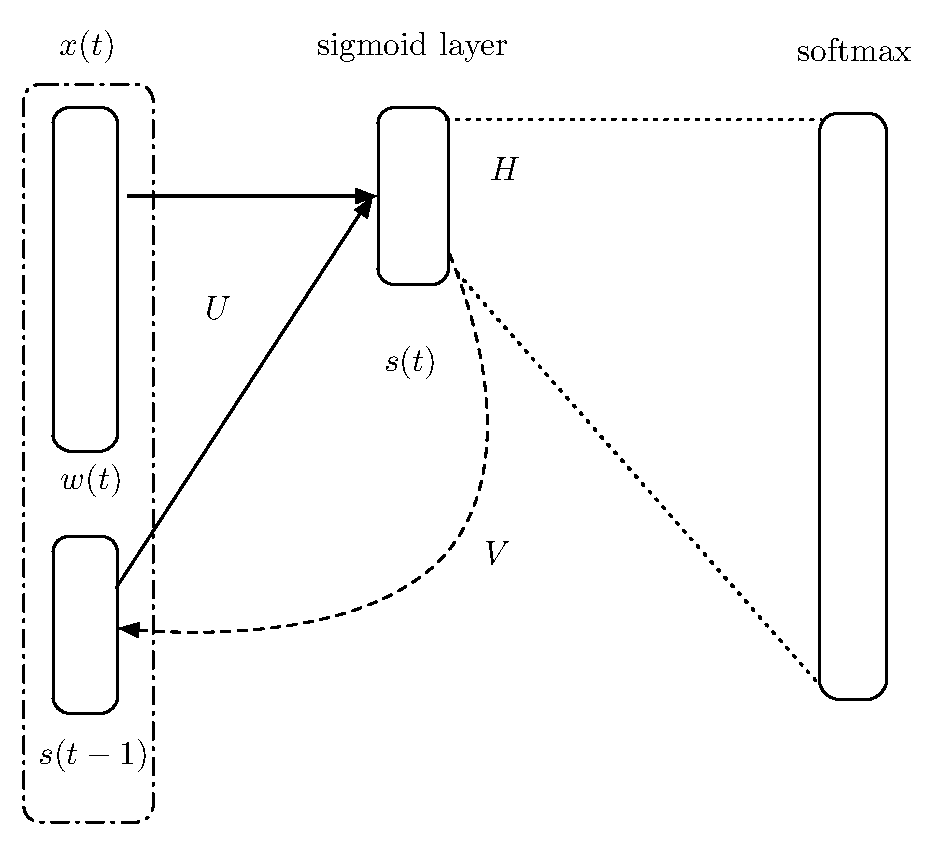
\includegraphics[width=0.6\textwidth]{images/mikolov-rnnlm.pdf} 
    \caption{Recurrent Neural Network Language Model Architecture}
    \label{fig:RNNLM_architecture}
\end{figure}



Figure \ref{fig:RNNLM_architecture} depicts the architecture of the simple
recurrent neural network. Similar to the \ac{FNNLM},    $w(t)$ represents the word in time $t$ encoded using 1-of-$V$ coding.  $s(t-1)$ represents the output values in the
hidden layer from the previous time step. Therefore $x(t)$, the input, has
the size of the vocabulary $V$ and of vector $s(t-1)$. After the network is
trained, the output represents the probability  in  equation
(\ref{eq:lm_probability})  \cite{mikolovphd2012}. % The network is trained
% using stochastic gradient descent using the
% \textit{backpropagation} algorithm \cite{conf/interspeech/MikolovKBCK10,Bishop:1995:NNP:525960}.


\subsubsection{Model Complexity}
\label{sec:sub:sub:mikolov_rnnlm_complexity}

Assuming that the hidden layer and the word representation share the same
dimensionality with the hidden layer, the complexity per training example of the \ac{RNNLM} model is
given by:


\begin{equation} Q = H \times H + H \times V,   \end{equation}

In a similar fashion to the \ac{FNNLM}, the term $H \times V$ can be
efficiently reduced to $H \times log_2(V)$ by using the hierarchical softmax
formulation. Thus, most of the complexity comes $H \times H$.

% Recurrent neural networks do not use limited size of con- text. By using recurrent connections, information can cycle in
% side these networks for arbitrarily long time (see [5]). However, it is also often claimed that learning long-term dependencies by stochastic gradient descent can be quite difficult [6].
% In our work, we have used an architecture that is usually called a simple recurrent neural network or Elman network [7]. This is probably the simplest possible version of recurrent neu- ral network, and very easy to implement and train. The network has an input layer x, hidden layer s (also called context layer or state) and output layer y. Input to the network in time t is x(t), output is denoted as y(t), and s(t) is state of the network (hidden layer). :




% A major deficiency of Bengio’s approach is that a feedfor- ward network has to use fixed length context that needs to be specified ad hoc before training. Usually this means that neural networks see only five to ten preceding words when predicting the next one. It is well known that humans can exploit longer context with great success. Also, cache models provide comple- mentary information to neural network models, so it is natural to think about a model that would encode temporal information implicitly for contexts with arbitrary lengths.


\subsection{Neural Network Language Model Proposed by Mikolov}
\label{sec:mikolov-neural-net-model}



The \ac{NNLM} proposed by Mikolov use a similar  approach to the
\ac{NNLM} described  in section \ref{subsec:fwd-neural-net-lm}. However, in  Mikolov's  model  the neural
network architecture is split in two steps. In the first section of  the
architecture  a bigram  neural network is trained. Given a word $w$ from a vocabulary $V$, the neural
network tries to estimate the the probability distribution of the next word
in the text. Both the input and output are of size $|V|$, were the words a
usually is encoded with 1-of-$K$ encoding, with $K=|V|$.  There is is one hidden layer of
size $|D|$. This layer is of  arbitrary size (reported by the authors  to
range from 20-60). As with other models, the output layer  is a  softmax
layer. The network is trained  using the standard \textit{backpropagation}
algorithm \cite{conf/icassp/MikolovKBGC09}. 

The second step consists of a  $N$-gram network. That is a network that tries to predict $w_t$ based on previous $N-1$ words. 
The network is trained in a 
similar way, however the input vector does not encode previous words using 1-of-$K$ encoding, but is formed using $N-1$ projections from
the  bigram network. These projections are the learned weights of dimension
$|D|$ learned by the big-gram network. Figure
\ref{fig:mikolov_nnlm_architecture} shows a schematic of the two-network architecture.


\subsubsection{Model Complexity}

As this model is composed of two parts, we then split the complexity
definition in two . One for the calculation of the bigram representation and
one for the final probability estimation:

\begin{equation} Q_1 = V \times D + D \times V  \end{equation}

\begin{equation} Q_2 =  N \times D \times H + H \times V   \end{equation}

\begin{equation} Q = Q_1 + Q_2
\end{equation}

With $Q_1$ and $Q_2$ the complexity of the bigram network and the $N$-gram
network respectively. Although not mentioned by the authors, efficiency
improvement can be achieved by using hierarchical formulations of the softmax. If used, most of the complexity  lies in the  $N \times D \times
H$ term of $Q_2$.

\begin{figure}[hptb!]
    \centering
    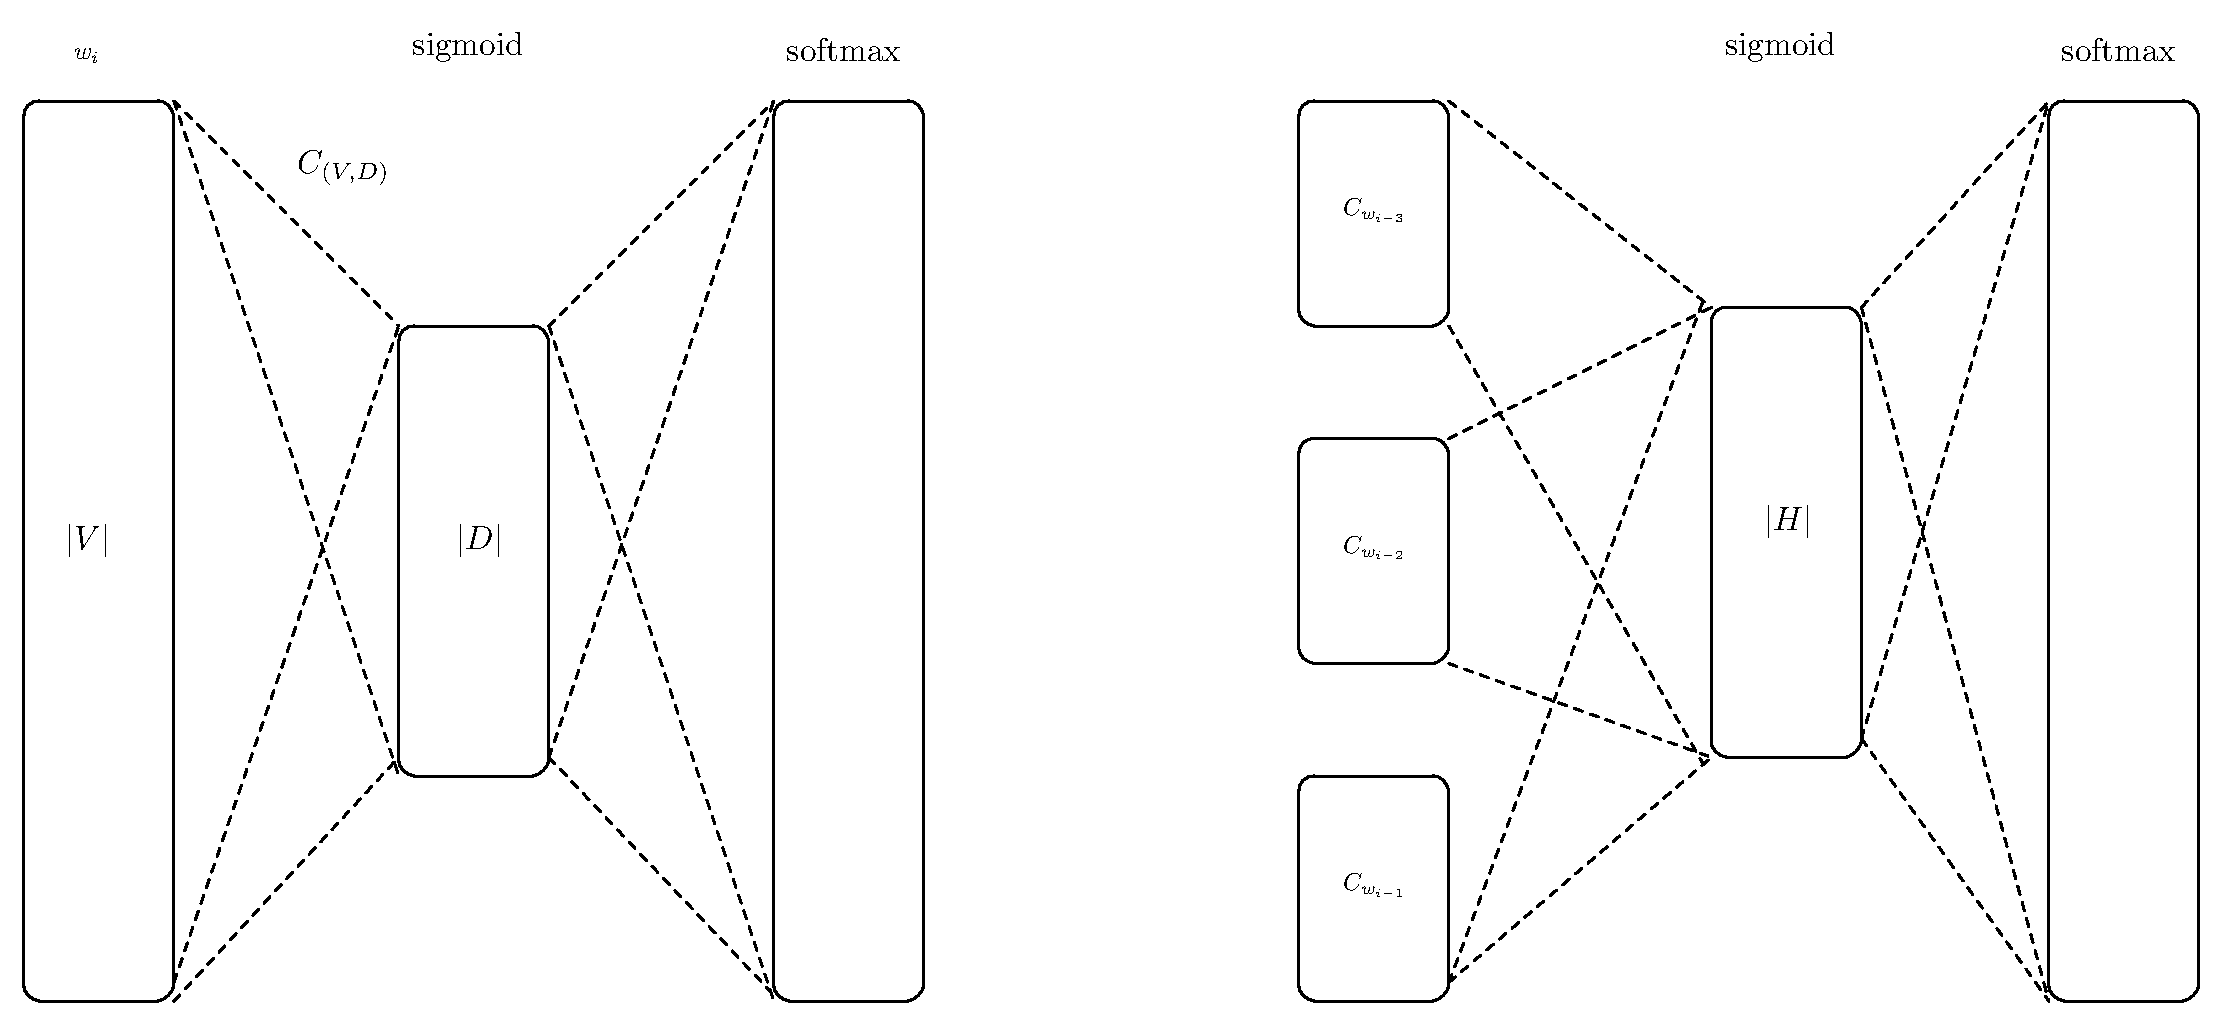
\includegraphics[width=1.0\textwidth]{images/mikolov-fnnl-latex.pdf} 
    \caption{Architecture of the \ac{NNLM} proposed by Mikolov.}
    \label{fig:mikolov_nnlm_architecture}
\end{figure}
  

% \subsection{Mikolov Neural Network Model}



% \section{Deep Learning}
% \label{sec:deep_learning}


% \section{Represenation of Text}
% \label{sec:rel_represenation_text}


% \subsection{Local Representations}
% \label{sec:rel_local_representation}

% \subsubsection{N-grams}
% \label{sec:sub_ngrams}

% \subsubsection{Bag-of-words}
% \label{sec:rel_bow}

% \subsubsection{1-of-N coding}
% \label{sec:1_of_coding}

% \subsection{Continuous Representations}
% \label{sec:sub_continuous_representation}

% \subsubsection{Latent Semantic Analysis}
% \label{sec:rel_local_representation}

% \subsubsection{Latent Dirichlet Allocation}
% \label{sec:rel_lda}

% \subsubsection{Distributed Representations}
% \label{sec:dis_rep}





%%% Local Variables: 
%%% mode: latex
%%% TeX-master: "../main.tex"
%%% End: